\documentclass{ctexart}
\CTEXsetup[format={\Large\bfseries}]{section}
\newcommand{\jn}{JN}
\usepackage{graphicx}
\usepackage{float}

\begin{document}

\title{学习笔记--istio}
\author{mayidudu 来自 \jn}
\maketitle
%https://blog.csdn.net/wcx1293296315/article/details/79775671, 插图
\tableofcontents


\begin{center}
	本篇笔记用于记录istio学习过程中遇到的问题
\end{center}
\section{ServiceMesh}
“Service Mesh”概念还非常年轻,这个词在国内被翻译为“服务网格”或“服务啮合层”,我们这里就用Service Mesh这个英文词。这里摘录一下ServiceMesh中文社区上的一篇名为《年度盘点2017之Service Mesh:群雄逐鹿烽烟起[1]》的文章中对Service Mesh概念的回顾:在 2016 年年初,“Service Mesh”还只是 Buoyant 公司的内部词汇,而之后,它开始逐步走向社区:2016 年 9 月 29 日在 SF Microservices 上,“Service Mesh”这个词汇第一次在公开场合被使用。这标志着“Service Mesh”这个词,从 Buoyant 公司走向社区。2016 年 10 月,Alex Leong 开始在 Buoyant 公司的官方 Blog 中连载系列文章“A Service Mesh for Kubernetes”。随着“The Services must Mesh”口号的喊出,Buoyant 和 Linkerd 开始 Service Mesh 概念的布道。2017 年 4 月 25 日,William Morgan 发布博文“What’s a Service Mesh? And why do I need one?”。正式给 Service Mesh 做了一个权威定义。而Service Mesh真正引起大家关注要源于istio项目的开源发布。该项目由Google、IBM共同合作创建,Lyft公司贡献了Envoy项目将作为Istio Service Mesh的data panel。Google、IBM的影响力让Service Mesh概念迅速传播,同时也让大家认识到了Istio项目在Service Mesh领域的重要性,于是纷纷选择积极支持并将自己的产品或项目与Istio项目集成。
Istio项目是Service Mesh概念的最新实现,旨在所有主流集群管理平台上提供Service Mesh层,初期以实现Kubernetes上的服务治理层为目标。

\section{istio是什么}
一个用来连接、管理和保护微服务的开放平台。 
Istio提供一种简单的方式来建立已部署服务网络,具备负载均衡、服务间认证、监控等功能,而不需要改动任何服务代码。
想要为服务增加对Istio的支持,您只需要在环境中部署一个sidecar,使用Istio控制面板功能配置和管理代理,拦截微服务之间的所有网络通信。


\section{istio的架构}
\begin{figure}[H]
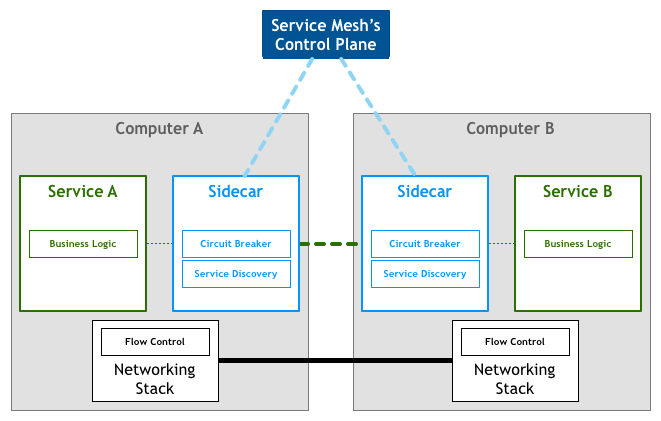
\includegraphics[scale=0.6]{istio/framework.png}
\caption{istio架构}
\end{figure}

\section{istio的主要功能}
流量管理(Pilot)。控制服务之间的流量和API调用的流向,使得调用更灵活可靠,并使网络在恶劣情况下更加健壮。

可观察性。通过集成zipkin等服务,快速了解服务之间的依赖关系,以及它们之间流量的本质和流向,从而提供快速识别问题的能力。

策略执行(mixer)。将组织策略应用于服务之间的互动,确保访问策略得以执行,资源在消费者之间良好分配。策略的更改是通过配置网格而不是修改应用程序代码。

服务身份和安全(Istio-auth)。为网格中的服务提供可验证身份,并提供保护服务流量的能力,使其可以在不同可信度的网络上流转。

除此之外,Istio针对可扩展性进行了设计,以满足不同的部署需要:

平台支持。Istio旨在可以在各种环境中运行,包括跨云、预置环境、Kubernetes、Mesos等。最初专注于Kubernetes,但很快将支持其他环境。
集成和定制。策略执行组件可以扩展和定制,以便与现有的ACL、日志、监控、配额、审核等解决方案集成。

\section{istio分层}
分为控制平面和数据平面两部分。 
\begin{enumerate}
	\item [-] 控制平面:Pilot, Mixer, Istio-Auth,分别对Istio中的服务做流量管理,策略配置,安全通信等规则配置 
	\item [-] 数据平面:所有pod上的Envoy,负责所有规则的执行
\end{enumerate}
\begin{figure}[H]
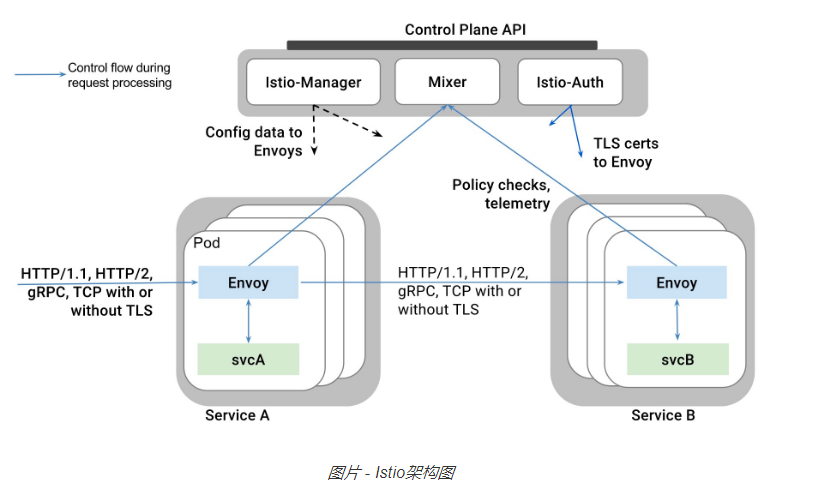
\includegraphics[scale=0.5]{istio/framework2.png}
\caption{istio分层结构}
\end{figure}
Sidecar中Envoy代理了Pod中真正业务Container的所有进出流量,并对这些流量按照控制平面设定的“治理逻辑”进行处理。而这一切对Pod中的业务应用是透明的,开发人员可以专心于业务逻辑,而无需再关心微服务治理的逻辑。Istio代表的Service Mesh的设计理念被认为是下一代“微服务统一框架”,甚至有人认为是微服务框架演化的终点。
Istio于2017年5月24日发布了0.1 release版本,目前已经到release1.1,并且已经部署在云平台,如华为云。

\section{基本概念}

\subsection{Traffic Management}
	使用 istio 的流量管理模型实质上解耦了 traffic flow 和 infrastructure scaling,
你可以通过 Pilot 指定 traffic 遵循的规则, 然后由 Pilot 和 Envoy 来做其余的事情,  而不是直接指定让哪个 Pods/VMs 接收 traffic.
\begin{enumerate}
	\item [*] \textbf{Pilot and Envoy:}
在 istio 中用于 traffic management 的核心组件就是 Pilot, 它管理和配置部署在 service mesh 中的 envoy.
Pilot 让你指定你想使用哪些规则来路由Envoy proxies 之间的 traffic , 并配置 failure recovery 特性,例如 timeouts, retries, circuit breakers.
它还维护一个网格中所有服务的 canonical model (规范模型) , 并且使用这个模型 让envoy实例 通过它的 discovery service 知道网格中的其他envoy实例的存在.
每个 envoy 实例都维护一份 load balancing 信息, 这份信息基于它从 Pilot 获取的信息, 并且周期性地对位于其 load-balancing pool 中的其他实例进行健康检查, 从而允许它可以在遵循指定的路由规则的同时也能智能地在目标实例之间分配流量.
Pilot 负责部署在服务网格中的 envoy实例 的生命周期.

	
	\item [*] \textbf{Request routing:}
	在istio中一个服务的模型和其在底层平台(例如kubernetes,Mesos,Cloud foundry(代工厂)等等)的表示形式无关.
	Platform-specific adapters 负责将 istio中的服务模型 polulating 到指定平台.
	istio 引进了 服务版本 的概念, 这可以区分不同版本的服务或不同环境的服务, 而且一般多哟用于 A/B测试 和 金丝雀发布.
	对于服务调用方而言, 它们不知道服务版本的存在. 它们面对的还是原来的服务,没有变化.  envoy 负责解析并转发 client 和 service 直接的请求和响应.
	envoy 可以根据你通过 Pilot 制定的路由规则 选择服务, 可以根据请求的 headers, 源/目的地的tags, 或者某个版本的weight 来进行路由.
	istio 不提供DNS, 应用可以尝试使用底层平台提供的DNS服务(例如 kube-dns, mesos-dns 等等)
	
	\item [*] \textbf{Ingress and egress:}
	istio 假设所有的进入和离开服务网格的流量 都是通过 envoy 代理的.
	istio 假设已经存在一个服务注册表用于追踪服务的 pods/VMs . istio 还假设一个服务的新实例会自动注册到服务注册表中, 并且不健康的实例会自动移除.  底层平台(例如kubernetes和Mesos)已经为基于容器的应用提供了这些功能, 并且基于VM的应用也有很多已经存在的解决方案.
	Pilot 消费服务注册表中的服务信息, 并提供一个平台无关的 服务发现接口.  服务网格中的envoy实例就从这个接口获取信息.
	
	\item [*] \textbf{handling failures:}
	envoy 提供了一套 out-of-the-box(开箱即用)的选项用于故障恢复功能,  这些功能包括:
	
	超时返回: Timeouts\\
	重试: Bounded retries with timeout budgets and variable jitter between retries\\
	到upstream服务的并发连接数和请求数限制: Limits on number of concurrent connections and requests to upstream services\\
	对负载均衡池中的服务的周期性的主动健康检查: Active (periodic) health checks on each member of the load balancing pool\\
	细粒度的断路器(被动的健康检查): Fine-grained circuit breakers (passive health checks) – applied per instance in the load balancing pool
	
	这些功能可以在 运行时 动态配置, 通过 istio 的 traffic management 的 rules.
	
	\item [*] \textbf{Fine tuning:}
	Istio’s traffic management rules 允许你设置每个服务的默认的 failure discovery, 和默认的服务版本.
	然而, 服务的消费者也可以通过特定的HTTP请求头 来覆盖默认的 timeout 和 重试次数, 在 envoy 作为proxy时,这些头是 x-envoy-upstream-rq-timeout-ms and x-envoy-max-retries .
	
	

\end{enumerate}

\section{应用领域}

\section{研究重点}



\begin{table}[h]
	\centering
	\caption{研究步骤}
	\begin{tabular}{|c|c|}
		\hline
		顺序 & \\\hline
		1 & \textbf{安装测试基本功能} \\\hline
		2 & \textbf{阅读源码} \\\hline
		3 & \textbf{能够进行编译} \\\hline
		4 & \textbf{了解基础架构并能够进行修改} \\\hline
	\end{tabular}
\end{table}

\begin{table}[h]
	\centering
	\caption{研究时间安排}
	\begin{tabular}{|c|c|}
		\hline
		2018-12-31 & 测试环境构建 \\\hline
		2019-01-15 & 了解基本的源码架构 \\\hline
	\end{tabular}
\end{table}

\section{istio测试环境}
\subsection{title}


\begin{table}[h]
	\centering
	\caption{测试环境}\label{tab:tab1}
	\begin{tabular}{|c|c|c|}
		\hline
		服务器 & 2个vm & fusion \\\hline
		OS & Centos7 & 固定硬盘 \\\hline
		Mem & 4G  & 支持Docker部署 \\
		\hline
	\end{tabular}
\end{table}


\section{istio与spring cloud比较}
istio是无侵入式的,可以支持多语言,而spring cloud是针对java平台的。

\section{问题}

\subsection{istio 服务无法访问外网问题}
缺省情况下,启用了Istio的服务是无法访问外部URL的,这是因为Pod中的iptables把所有外发传输都转向到了Sidecar代理,而这一代理只处理集群内的访问目标。

我们可在Istio集群中使用两种方式来访问外部服务:
使用Egress规则。
配置Istio Sidecar,在他的iptables中排除对外部IP的控制。 
Egress 规则
配置Istio Sidecar 
让指定IP范围直接穿透Istio,就需对源服务的Envoy Sidecar进行配置,阻止其对外部请求的拦截。

通过--includeIPRanges指定。

% kubectl apply -f <(istioctl kube-inject -f samples/sleep/sleep.yaml --includeIPRanges=10.0.0.1/24)

%IPranges即service的IP范围,在kube-api_server.service中通过–service-cluster-ip-range指定。

\end{document}